\documentclass[a4paper]{article}

\usepackage[english]{babel}
\usepackage[utf8x]{inputenc}
\usepackage{amsmath}
\usepackage{graphicx}
\usepackage[colorinlistoftodos]{todonotes}
\usepackage{schemabloc}
\usetikzlibrary{calc}

\newcommand{\mb}[1]{\mathbf{#1}}
\newcommand{\derivt}[1]{\frac{\mathrm{d}#1}{\mathrm{dt}}}
\newcommand{\deriv}[2]{\frac{\partial#1}{\partial#2}}

\PassOptionsToPackage{hyphens}{url}\usepackage[colorlinks=true,urlcolor=blue]{hyperref}
\urlstyle{same}
\sloppy

\title{AMORO Lab Part 3: Simulation of a Biglide mechanism}
\author{Damien SIX\\ damien.six@ls2n.fr}
\date{Released: August 20, 2021}

\begin{document}
\maketitle
\begin{figure}[h!]
\centering
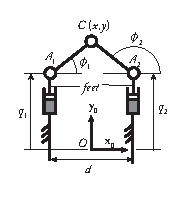
\includegraphics[width=0.6\textwidth]{PuRRRPu.eps}
\caption{Kinematic model of the Biglide. The prismatic joints are actuated.}
\label{fig:biglide}
\end{figure}
\section{Objective}
The main objective of the present lab is to compute the geometric, kinematic and dynamic models of a Biglide mechanism and to compare them with the results obtained with GAZEBO. Then, a controller will be designed to track a trajectory in simulation.

The kinematic architecture of the Biglide is shown in Fig.\ref{fig:biglide}. For the mechanism of the Gazebo mock-up, the geometric parameters are: 
\begin{itemize}
\item    $d=0.4$ m
\item    $l_{A1C}=0.2828427$ m
\item    $l_{A2C}=0.2828427$ m
\end{itemize}
and the base dynamic parameters are:
The base dynamic parameters are: 
\begin{itemize}
\item $m_p$ = 3 kg the mass of the end-effector
\item $m_f$ = 1 kg the mass of each foot
\end{itemize} 

\section{Evaluation}
The deliverable for this lab is a zip file containing:
\begin{itemize}
	\item A detailed computation of the biglide mechanism models (PDF file).
	\item A detailed report (with comment, figures, etc.) of your work (PDF file). Concerning figures, the scripts output scopes that allow you to check the validity of your models. They are here to help you during the lab. Please do not use them directly in your final report and take the time to make nicer plots with the correct labels, scales, etc. (no lazy print screen). Learning how to make nice figures is also part of your training.
	\item The \textit{biglide\_models.py} file: all models should match with Gazebo simulation. The input-output of the functions in \textit{biglide\_models.py} must not be modified from the original file.
	\item The \textit{control.py} file: when launched, the file must perform the desired trajectory using computed torque control.
\end{itemize}
This report is the main way to have a clear feedback about your work, so its quality and content will have a great impact on the final grade. Your work must be clearly detailed and commented.

The script files will be tested and their effectiveness will also be part of the grade. To be evaluated your file must be free of any error. You can test if your models pass the evaluation process by running the model\_eval.py script.

After the end of the four lab sessions, you have \textbf{two weeks} to upload the deliverable as a .zip file at the following address  \href{https://www.dropbox.com/request/AgEcJ96a4b1EdvbEftot}{https://www.dropbox.com/request/AgEcJ96a4b1EdvbEftot}.

\section{Models of the Biglide}
\label{analysis}
Compute and compare with the Gazebo simulation the following models of the Biglide.
%
All the following models must be validated
\begin{itemize}
    \item The Direct Geometric Model
    \item The Direct Geometric Model for passive joints
    \item The Inverse Geometric Model
    \item The First Order Kinematic Model
    \item The First Order Kinematic Model for passive joints
    \item The Inverse First Order Kinematic Model
    \item The Second Order Kinematic Model
    \item The Second Order Kinematic Model for passive joints
    \item The Inverse Second Order Kinematic Model
    \item The inverse Dynamic Model
\end{itemize}
%
All your model should be filled in the \textit{biglide\_models.py} file without changing the input-output of the pre-defined functions.
%
\section{Computed Torque Control simulation}

Using the Robot class input and output, code in \textit{control.py} a computed torque control to track a desired trajectory. The trajectory should start from the robot initial position and reach the point x=0.05, y=0.7 in 2.0 seconds.
    
\section{Crossing type 2 singularities (bonus points)}
\begin{itemize}
    \item Design a trajectory that crosses a type 2 singularity for this robot.
    \item What happen when you try to track this trajectory using a computed torque control law?
    \item Design a trajectory that can cross safely the type 2 singularity. Display the theoretical torque inputs for this trajectory using the inverse Dynamic Model.
    \item Try to track this trajectory using Gazebo and the computed torque control. What happen (and why)?
\end{itemize}
%
The file \textit{control.py} provided with your final report must perform the tracking of a trajectory using computed torque control as asked in section 4. Please use an other script for the trials with the type 2 singularity.
%
\end{document}
  




